\documentclass[a4paper]{extarticle}
\usepackage[utf8]{inputenc}
\usepackage[a4paper, margin=1in]{geometry}

\usepackage{amssymb}
\usepackage{amsmath}
\usepackage{enumitem}
\usepackage{tcolorbox}
\usepackage{fancyhdr}
\usepackage{graphicx}
\usepackage{float}

\setlength{\parindent}{0em}
\setlength{\parskip}{0.4em}

\definecolor{theoremblue}{RGB}{1, 73, 124}
\definecolor{corollaryblue}{RGB}{70, 143, 175}
\definecolor{exampleblue}{RGB}{137, 194, 217}

\newtcolorbox{tbox}{colback=theoremblue!20,colframe=theoremblue,
boxrule=0pt,arc=0pt,boxsep=2pt,left=2pt,right=2pt,leftrule=2pt}

\newtcolorbox{cbox}{colback=corollaryblue!20,colframe=corollaryblue,
boxrule=0pt,arc=0pt,boxsep=2pt,left=2pt,right=2pt,leftrule=2pt}

\newtcolorbox{ebox}{colback=exampleblue!20,colframe=exampleblue,
boxrule=0pt,arc=0pt,boxsep=2pt,left=2pt,right=2pt,leftrule=2pt}

\title{EnpRisk - Lecture Notes Week 9}
\author{Ruben Schenk, ruben.schenk@inf.ethz.ch}
\date{\today}

\pagestyle{fancy}
\fancyhf{}
\rhead{ruben.schenk@inf.ethz.ch}
\rfoot{Page \thepage}
\lhead{EnpRisk - Lecture Notes Week 9}

\begin{document}

\maketitle

\subsection{The Golden Age (1947-1968)}

The \textbf{Golden Age} (1947-1968) describes the two decades after WWII, which were blessed with \textit{extraordinary economic growth:}

\begin{itemize}
    \item Mean reversion: Recovery of the economy to its full potential after WWII
    \item Stimulus: Reconstruction of infrastructure and industry
    \item Productivity: Increase from technical innovations and capital investments
\end{itemize}

There was a \textit{social contract} between workers and owners on:

\begin{itemize}
    \item The parallel growth of real wages and Productivity
    \item The ensuring that fruits of the economic progress were equitably shared
    \item This led to wealth accumulation and spare time, which in turn led to \textbf{consumerism}
\end{itemize}

The first shift led to a collapse of inequality, which stayed low during the Golden Age. If we define $r$ to be the pure rate of return to capital, and $g$ the growth rate of world output, then T. Piketty (2014) stated that $r < g$ leads to inequality. However, our proposition is that inequality leads to $r > g$.

Free time and wealth accumulation created a \textit{consumer society} with new demand for consumer goods like electrical apparel, automobiles and entertainment services.

\subsection{The Second Shift (1969-1979)}

The \textbf{Second Shift} (1969-1979) was a direct consequence of the Nixon shock and the end of Bretton Woods (1971):

\begin{itemize}
    \item At a certain point there were more dollars in the hands of foreign countries (so-called eurodollars) than the total gold stock of the US
    \item Trust in the US Dollars, which was the keystone of the Bretton Woods system, evaporated
    \item Whereas the gold reserves of the US were reduced from 65\% (1952) to 29\% (1967), the opposite happened in Europe, where the gold reserves went from 6\% (1952) to 26\%(1967)
    \item This dynamic ended in 1971 with the \textit{Nixon Shock}, when the US President Nixon unilaterally ended the convertibility of the Dollars to gold. This was the end of the Bretton Woods system
\end{itemize}

\subsection{The Fool's Golden Age (1980-2019)}

The \textbf{Fool's Golden Age} may also be described as the illusion of the perpetual money machine:

\begin{itemize}
    \item Consumption, not founded by savings but by debt, and by wealth extracted from the stock and the housing market
    \item Economic growth, not driven by productivity increase in the real economy, but by growth of the financial sector
    \item Further supported by a climate of deregulation and a massive growth in financial derivatives
    \item Resulting in a succession of bubbles and crashes, feeding upon each other and culminating the CFG of 2008
\end{itemize}

This Age is mainly plagued by decreased savings and increased consumption based on debt:

\begin{figure}[H]
    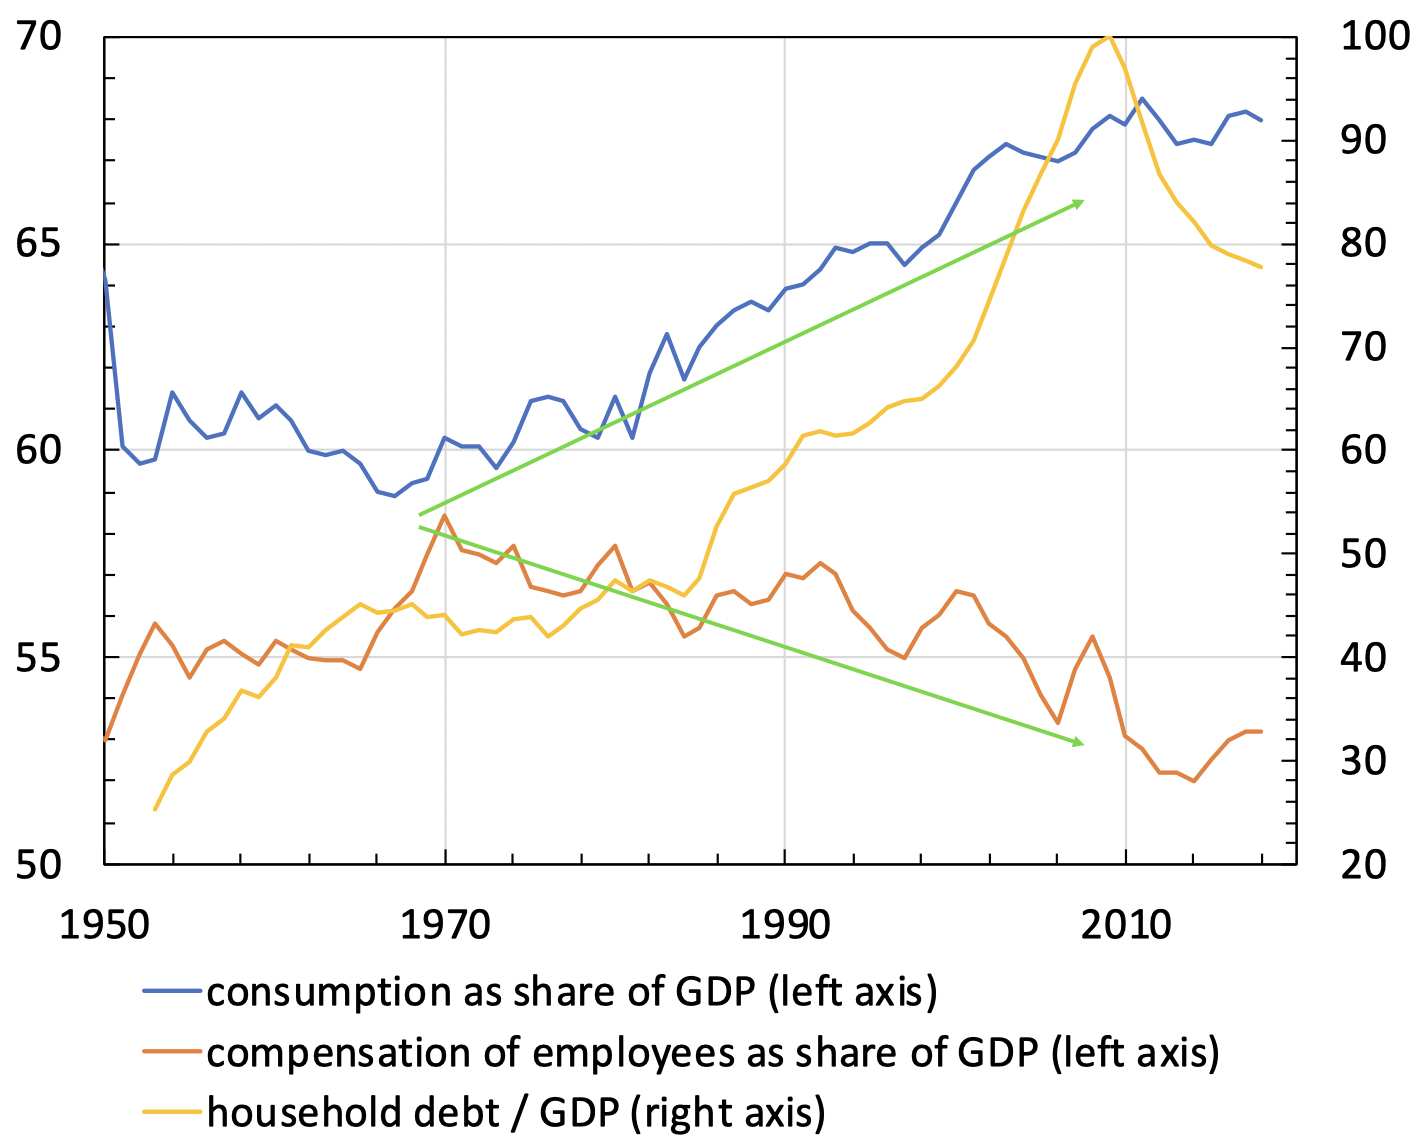
\includegraphics[width=11cm]{../images/EnpRisk_Fig9-1}
    \centering
\end{figure}

\textbf{Globalization} is not an inevitable process, and it is also not a linear process:

\begin{itemize}
    \item The \textit{first wave} came with the technological revolution, pushed forward by increased connectivity, falling transportation costs and the gold standard that created a global marketplace
    \item The \textit{second wave} renewed international cooperation and trade liberalization after nationalism during the First Shift brought globalization back to its previous level.
    \item In the \textit{third wave,} new information and communication systems made it possible to manage and control geographically dispersed supply chains. 
\end{itemize}

Another characteristic of the Fool's Golden Age is the massive increase in debt, but the remarkable decrease in the efficiency of debt. Now one dollar of debt in the non-financial sector generates 25 cents in GDP. In other words, this increase in debt is not used to increase investment in tangible assets.

Consumption has still increased since the Golden Age, but the mix shifted from goods to services (such as healthcare, pension, financial services, insurance, etc.).

\begin{figure}[H]
    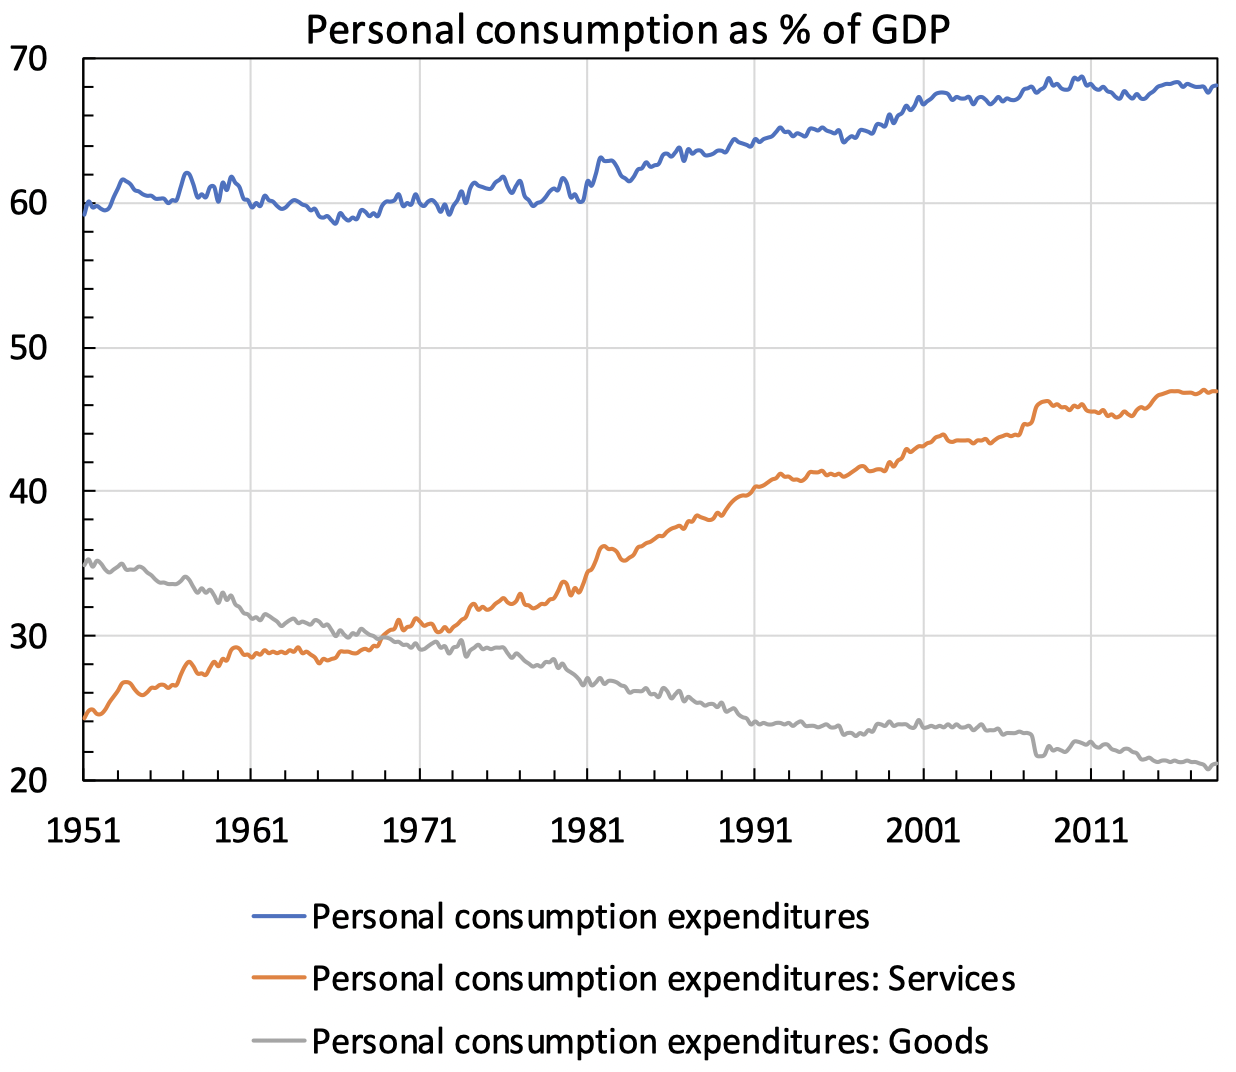
\includegraphics[width=11cm]{../images/EnpRisk_Fig9-2}
    \centering
\end{figure}

\end{document}